\subsection{Orbit membership: independent graph audit and paired timings}

The eleven focused tests pass.  An exhaustive audit covers all systems with at most two interval generators
on universes of size at most five, up to input-generator order: $7{,}398$
indices across both merger rules and $34{,}026$ literal point checks.
The random audit prepares indices for $3{,}200$ random
interval relations under both maintained merger rules, giving $6{,}400$
checked indices and $208{,}000$ literal minimum comparisons.  A union-find
oracle explicitly expands only these bounded test inputs.  It also checks
$64{,}000$ sampled pair queries and all selected representatives, and all six
trace event types occur. The exhaustive and random tests also check the
complete canonical minimum interval set, sorted selection and ranks against
the literal graph. Two deliberately different valid traces establish
the distinction between canonical minimum labels and emission ordinals.

The geometric audit uses $67$ supplied normal vectors: parallel meridians
in one through ten tetrahedra and compatible mixtures of an interior
vertex sphere, a boundary vertex disc, and a one-sided M\"obius band in a
four-tetrahedron solid torus.  Both surface and boundary arc graphs are
tested under both merger rules, giving $268$ indices and another $73{,}528$
literal minimum comparisons.  These checks use the maintained exact
normal-coordinate adapter, with no native topology package required.
Separate tests cover $16{,}000$--$20{,}000$-bit endpoints, malformed and
unfinished proofs, source rebinding, caller mutation, disabled producer
entry points, and cancellation through false-valued callable objects.  A
separate exact fixture has $512$ disjoint minimum intervals and a $4{,}107$-bit
universe; its component count has $4{,}106$ bits, and the predicted $g=512$
interval bound is attained without enumerating components.

The portable paired benchmark has ten workloads, five shuffled arms,
one excluded warmup and seven measured rounds.  Single-query cases are
batched three times.  This gives $490$ measured complete arm calls and
$70$ warmup calls.  The compiled arm includes discovery, independent
verification, compilation and all requested comparisons.  The comparison
baseline shares the initial count and uses exact connected and singleton
shortcuts; only unresolved comparisons require augmented count schedules.
The original two-count API and identical controls are retained as separate
arms.  Every answer is compared outside the timer.

\begin{table}[htbp]
\centering
\caption{Complete repeated-membership workloads on supplied interval relations.
Discovery, independent verification, construction, and all queries are timed.
Times are milliseconds; ratios are paired medians.}
\label{tab:orbit-membership}
% Generated by generate_artifacts.py; edit the source JSON or generator.
\begingroup
\small
\setlength{\tabcolsep}{5pt}
\renewcommand{\arraystretch}{1.12}
\begin{tabular}{@{}p{6.5cm}rrrr@{}}
\toprule
Supplied relation & $q$ & Shared (ms) & Compiled (ms) & Ratio \\
\midrule
Meridian, $t=8$, scale $2^{512}+1$ & 1 & 2.845 & 2.993 & 0.925 \\
Meridian, $t=8$, scale $2^{512}+1$ & 8 & 12.880 & 2.852 & 4.582 \\
Meridian, $t=8$, scale $2^{512}+1$ & 32 & 46.957 & 2.996 & 15.629 \\
Meridian, $t=24$, scale $2^{128}+1$ & 1 & 25.157 & 20.437 & 1.224 \\
Meridian, $t=24$, scale $2^{128}+1$ & 8 & 111.298 & 20.308 & 5.502 \\
Meridian, $t=24$, scale $2^{128}+1$ & 32 & 422.509 & 20.539 & 20.686 \\
Primitive meridian, $t=8$ & 32 & 1.231 & 2.546 & 0.461 \\
M\"obius band, scale $2^{1024}+1$ & 32 & 1.540 & 0.321 & 4.447 \\
Four-tetrahedron compatible mixture & 32 & 29.527 & 2.124 & 13.915 \\
64-pair periodic chain & 32 & 14.182 & 1.629 & 8.757 \\
\bottomrule
\end{tabular}
\endgroup

\end{table}


\begin{figure}[htbp]
\centering
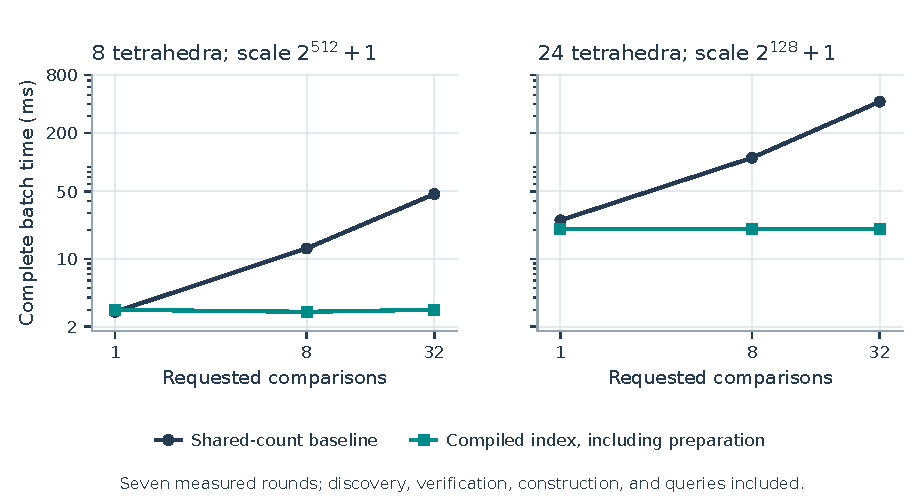
\includegraphics[width=\linewidth]{figures/orbit_queries.pdf}
\caption{Total membership-batch time as the number of requested comparisons
increases. Both compiled curves include preparation. No asymptotic law is
estimated from these finite observations.}
\label{fig:orbit-queries}
\end{figure}

Times are separate medians; the ratio is the median of paired ratios and
need not equal their quotient.  For the eight-tetrahedron source, the full
trace has $128$ events but the query program has $13$ point steps.  For
$24$ tetrahedra these figures are $832$ and $29$.  The periodic chain
compiles $65$ trace events to two point steps.  These are exact reductions
in work representation, independent of timer variation.

The primitive meridian is a necessary control: its first count proves the
relation connected, so the shared baseline answers all comparisons
immediately and is faster than index preparation.  The single-query
eight-tetrahedron case likewise shows no improvement.  Across all cases,
identical shared-control ratios range from $0.959$ to $1.040$, and
identical compiled-control ratios range from $0.969$ to $1.050$.  Thus the
large repeated-query effects are supported, while small percentage
differences should not be overinterpreted.

Raw records, inputs, query points, expected answers, reduction counts,
all shuffled arm orders and timings, and pre/post source hashes are in
\path{results/orbit_index.json}.  Audit evidence is in
\path{results/orbit_index_audit.json}; the portable drivers are in
\path{orbit_index_research/}.  Earlier prototype timings are not mixed into this table. Normal triangulation creation,
vector construction and conversion to interval relations are outside every
timer.  These results measure repeated queries on a supplied interval system,
not complete normal-surface calls or unknot-recognition runtime.
\subsection{Prepared canonical rank and selection}

The additional lookup experiment uses the sharp family of disjoint paired
blocks.  A supplied deterministic right-to-left trace is independently
verified before any query is timed.  The canonical minimum intervals and
every queried answer are checked against the direct block formulas, including
the conversion between emission ordinal and increasing-minimum rank.  Both
selection arms request the same original representatives on the same prepared
index; their numerical ordinal arguments differ because the orders differ.

Each measured call contains $512$ lookups, batched three times.  There are
seven shuffled measured rounds, one excluded warmup, and identical controls
for canonical rank and canonical selection.  Index construction is reported
separately and excluded from every lookup timer.  The original trace-ordinal
selection method reverses contractions; the canonical method searches the
compact minimum-interval union.

\begin{table}[htbp]
\centering
\caption{Prepared representative selection: 512 queries per call. Both selection
arms return the same source minima using their corresponding ordinals.
Preparation is excluded here and reported in the text. Times are milliseconds.}
\label{tab:orbit-rank}
% Generated by generate_artifacts.py; edit the source JSON or generator.
\begingroup
\small
\setlength{\tabcolsep}{5pt}
\renewcommand{\arraystretch}{1.12}
\begin{tabular}{@{}rrrrrr@{}}
\toprule
\shortstack{Minimum\\intervals} & \shortstack{Endpoint\\bits} & \shortstack{Emission\\(ms)} & \shortstack{Canonical\\(ms)} & Ratio & \shortstack{Rank\\(ms)} \\
\midrule
1 & 130 & 0.218 & 0.123 & 1.756 & 0.154 \\
16 & 134 & 0.794 & 0.138 & 5.922 & 0.168 \\
128 & 4105 & 7.600 & 0.327 & 23.791 & 0.348 \\
512 & 4107 & 29.732 & 0.365 & 81.511 & 0.408 \\
\bottomrule
\end{tabular}
\endgroup

\end{table}


All times concern a complete $512$-query call.  Preparation took respectively
$0.101$, $0.863$, $37.003$ and $557.962$ milliseconds in separately recorded
single observations.  Thus the submillisecond prepared lookup times do not
describe construction of the index.  Identical canonical-selection control
ratios range from $1.007$ to $1.034$, and rank-control ratios from $0.977$ to
$1.026$.  The final case has $512(2^{4096}+3)$ components while storing just
$512$ minimum intervals.  The bit-complexity conclusion is logarithmic in
the number of stored intervals, with binary-integer and output costs charged;
the finite timings are not a constant-time claim.

Full inputs, queried canonical ranks and corresponding emission ordinals,
analytic expected minima, source hashes, certificate hashes and all raw
samples are retained in \path{results/orbit_rank_select.json}.  The standalone
driver is \path{orbit_index_research/rank_select.py}.  This experiment measures
prepared representative lookups, separately from the preceding complete
membership-batch benchmark and from all unknot-recognition work.
